\documentclass[runningheads,a4paper]{llncs}

\usepackage[T1]{fontenc}
\usepackage{amsmath,amssymb}
\usepackage{booktabs}
\usepackage{graphicx}
\usepackage{array}
\usepackage{multirow}
\usepackage{url}
\usepackage{tikz}
\usepackage{placeins}
\usepackage{float}
\usetikzlibrary{arrows.meta,positioning,shapes.geometric}
\emergencystretch=2em
\setlength{\textfloatsep}{8pt plus 2pt minus 2pt}
\setlength{\floatsep}{8pt plus 2pt minus 2pt}
\setlength{\intextsep}{8pt plus 2pt minus 2pt}
\makeatletter
\setlength{\@fptop}{0pt}
\setlength{\@fpsep}{8pt plus 0pt minus 2pt}
\setlength{\@fpbot}{0pt plus 1fil}
\makeatother

\newcommand{\method}{TCVM-Net}
\newcommand{\dataset}{AdvTraffic-26}
\newcolumntype{L}[1]{>{\raggedright\arraybackslash}p{#1}}

\begin{document}

\title{TCVM-Net: Temporal Consistency Verification for Robust Traffic Surveillance Under Physical-Style Adversarial Attacks}
\titlerunning{Temporal Consistency Defense for Traffic Surveillance}

\author{Anonymous Authors}
\authorrunning{Anonymous}
\institute{Anonymous Institution}

\maketitle
\begin{abstract}
Traffic surveillance systems increasingly rely on real-time detectors for helmet compliance and rider monitoring, yet most adversarial defenses are evaluated under isolated-image assumptions. Physical-style perturbations can instead produce video-level failure patterns, including short confidence collapse, localization jumps, and object disappearance across adjacent frames. We propose \method, a lightweight YOLOv8 verification layer that treats track-level temporal inconsistency as adversarial evidence without modifying the detector. The verifier combines confidence stability, motion continuity, compact feature similarity, detector-count collapse gating, and short-gap recovery. YOLOv8n reaches 0.628 mAP@50 and 0.415 mAP@50:95 on the 750-image held-out helmet test set. On a paired 50-image subset, PGD attains 0.988 ASR and lowers mAP@50 from 0.675 to 0.229; reflective and occlusion attacks lower it to 0.152 and 0.216. On a controlled reflective video sequence, \method{} improves mAP@50 from 0.838 to 0.944 with 0.958 anomaly accuracy. On a 30-clip public HELMET benchmark with 720 human-annotated frames, clip-disjoint calibration reaches 0.887 held-out anomaly F1 at 0.021 FPR, while 20 fixed resplits yield median F1/FPR of 0.889/0.020. The threshold transfers unchanged to reflective attacks. A calibration-only detector patch reaches 0.406 held-out ASR but only 0.103 anomaly F1, exposing a temporally smooth failure mode. Edge profiling shows scaled-flow \method{} running at 14.10 FPS on the expanded calibrated benchmark.
\keywords{Adversarial Learning \and Traffic Surveillance \and YOLOv8 \and Temporal Consistency \and Physical Adversarial Attacks \and Robust AI}
\end{abstract}

\section{Introduction}

Intelligent transportation systems increasingly use deep object detectors for helmet compliance, rider detection, lane-use analysis, and violation screening. YOLO-family models offer a practical accuracy--latency trade-off for roadside cameras and edge units, but missed helmet or rider detections can affect enforcement, risk analytics, and downstream screening.

The same visual sensitivity that enables high-speed detection also exposes traffic models to physical manipulation. Stickers, reflective tape, partial occlusion, low light, and motion blur can suppress confidence or redirect attention even while the target remains visible, producing safety-relevant false negatives.

Most adversarial defenses assume isolated images. Preprocessing may suppress perturbation artifacts and adversarial training may improve robustness to attack families seen during training, but neither exploits the ordered stream already available in surveillance. Across nearby frames, helmets, riders, and motorcycles normally exhibit locally smooth motion, gradual confidence variation, and stable appearance. Physical-style attacks can instead induce abrupt confidence drops, localization jumps, feature discontinuity, or implausible disappearance.

\method{} wraps YOLOv8 and a tracker, scores confidence, motion, appearance, and disappearance over short histories, and rejects or recovers inconsistent predictions using a calibrated threshold. Recovery uses the recent track prior only for short gaps and discounts its confidence to avoid treating an inferred box as a normal observation. The method is a practical video-surveillance verification layer, not a certified defense.

The main contributions are:
\begin{enumerate}
    \item A modular temporal consistency verifier for adversarially robust traffic video.
    \item Lightweight anomaly scoring that combines confidence, motion, appearance, and disappearance evidence without retraining the detector.
    \item A reproducible helmet-surveillance benchmark covering eight digital and physical-style perturbation families.
    \item Evaluation against clean detectors, image preprocessing, adversarial augmentation, tracker-only recovery, and an ADAV-style reference baseline, including explainability and deployment costs.
\end{enumerate}

Unlike image preprocessing, matched augmentation, or tracker-only smoothing, \method{} combines several temporal inconsistencies as a post-inference security signal. Its contribution is an incremental but practical robustness layer for ordered traffic video; the experiments and limitations state this claim boundary explicitly.

\section{Related Work}

FGSM exposed sensitivity to small perturbations \cite{goodfellow2015explaining}, and PGD adversarial training became a strong first-order baseline \cite{madry2018towards}. Digital-norm robustness does not ensure physical robustness: EOT captures viewpoint, scale, lighting, and printability \cite{athalye2018synthesizing}, while traffic-sign attacks demonstrated road-scene risk \cite{eykholt2018robust}.

Localized universal patches can hide safety-critical objects \cite{brown2017adversarial}. APRICOT benchmarks physical patches on object detectors, while REAP adds road-scene geometry and lighting transformations \cite{braunegg2020apricot,hingun2023reap}; a recent survey details pose, illumination, sensor, and deployment constraints \cite{wei2026physical}. New attacks target traffic signs, printed traffic lights, nighttime reflectors, and Ultralytics YOLO under edge constraints \cite{xu2026naradv,pavlitska2025foolstoplight,suo2026rdpa,gala2025yolopatch}. AntiStyler, PBCAT, and PatchBlock improve patch robustness through retraining or image-level suppression, although unified evaluation still finds adaptive gaps \cite{yankelev2026antistyler,li2025pbcat,chattopadhyay2026patchblock,zheng2025revisiting}. These defenses primarily reason over individual images or estimated patch masks rather than whether detector behavior remains plausible over traffic video.

Temporal structure can expose attacks and create new attack surfaces. AdvIT detects adversarial frames through consistency \cite{xiao2019advit}; Themis removes localized regions in real-time video detection \cite{han2024themis}; and ADAV combines previous-frame consistency with attribution for object-vanishing patches on BDD100K \cite{mu2025adav}. PapMOT and structured video attacks show that patches can degrade association or suppress detections across frames \cite{long2024papmot,jacob2025structured}. Using edge-oriented YOLOv8 \cite{jocher2023ultralytics} and ByteTrack association \cite{zhang2022bytetrack}, \method{} specializes this insight to helmet/rider surveillance and combines track-level cues rather than relying only on reference-frame disappearance.

The distinction is architectural and empirical. AdvIT detects adversarial frames through adjacent prediction consistency but does not formulate track-level multi-cue recovery for helmet surveillance. Themis seeks and removes a localized adversarial region, whereas ADAV-style recovery emphasizes attribution and a stable reference frame. \method{} requires neither patch localization nor detector retraining; it fuses four inexpensive track-history signals and exposes both recovery and rejection decisions. Our ADAV-style comparator is retained because abrupt disappearance is the strongest case for reference-frame recovery, while the component ablation tests whether motion and appearance reduce false alarms beyond tracking alone.

\section{Proposed Methodology}

\subsection{System Overview}
Figure~\ref{fig:architecture} shows framewise YOLOv8 detection, ByteTrack association, temporal verification, and final prediction. The verifier does not alter detector weights and can wrap another framewise detector; YOLOv8 is used as the practical edge-oriented backbone throughout the experiments.

\begin{figure}[t]
\centering
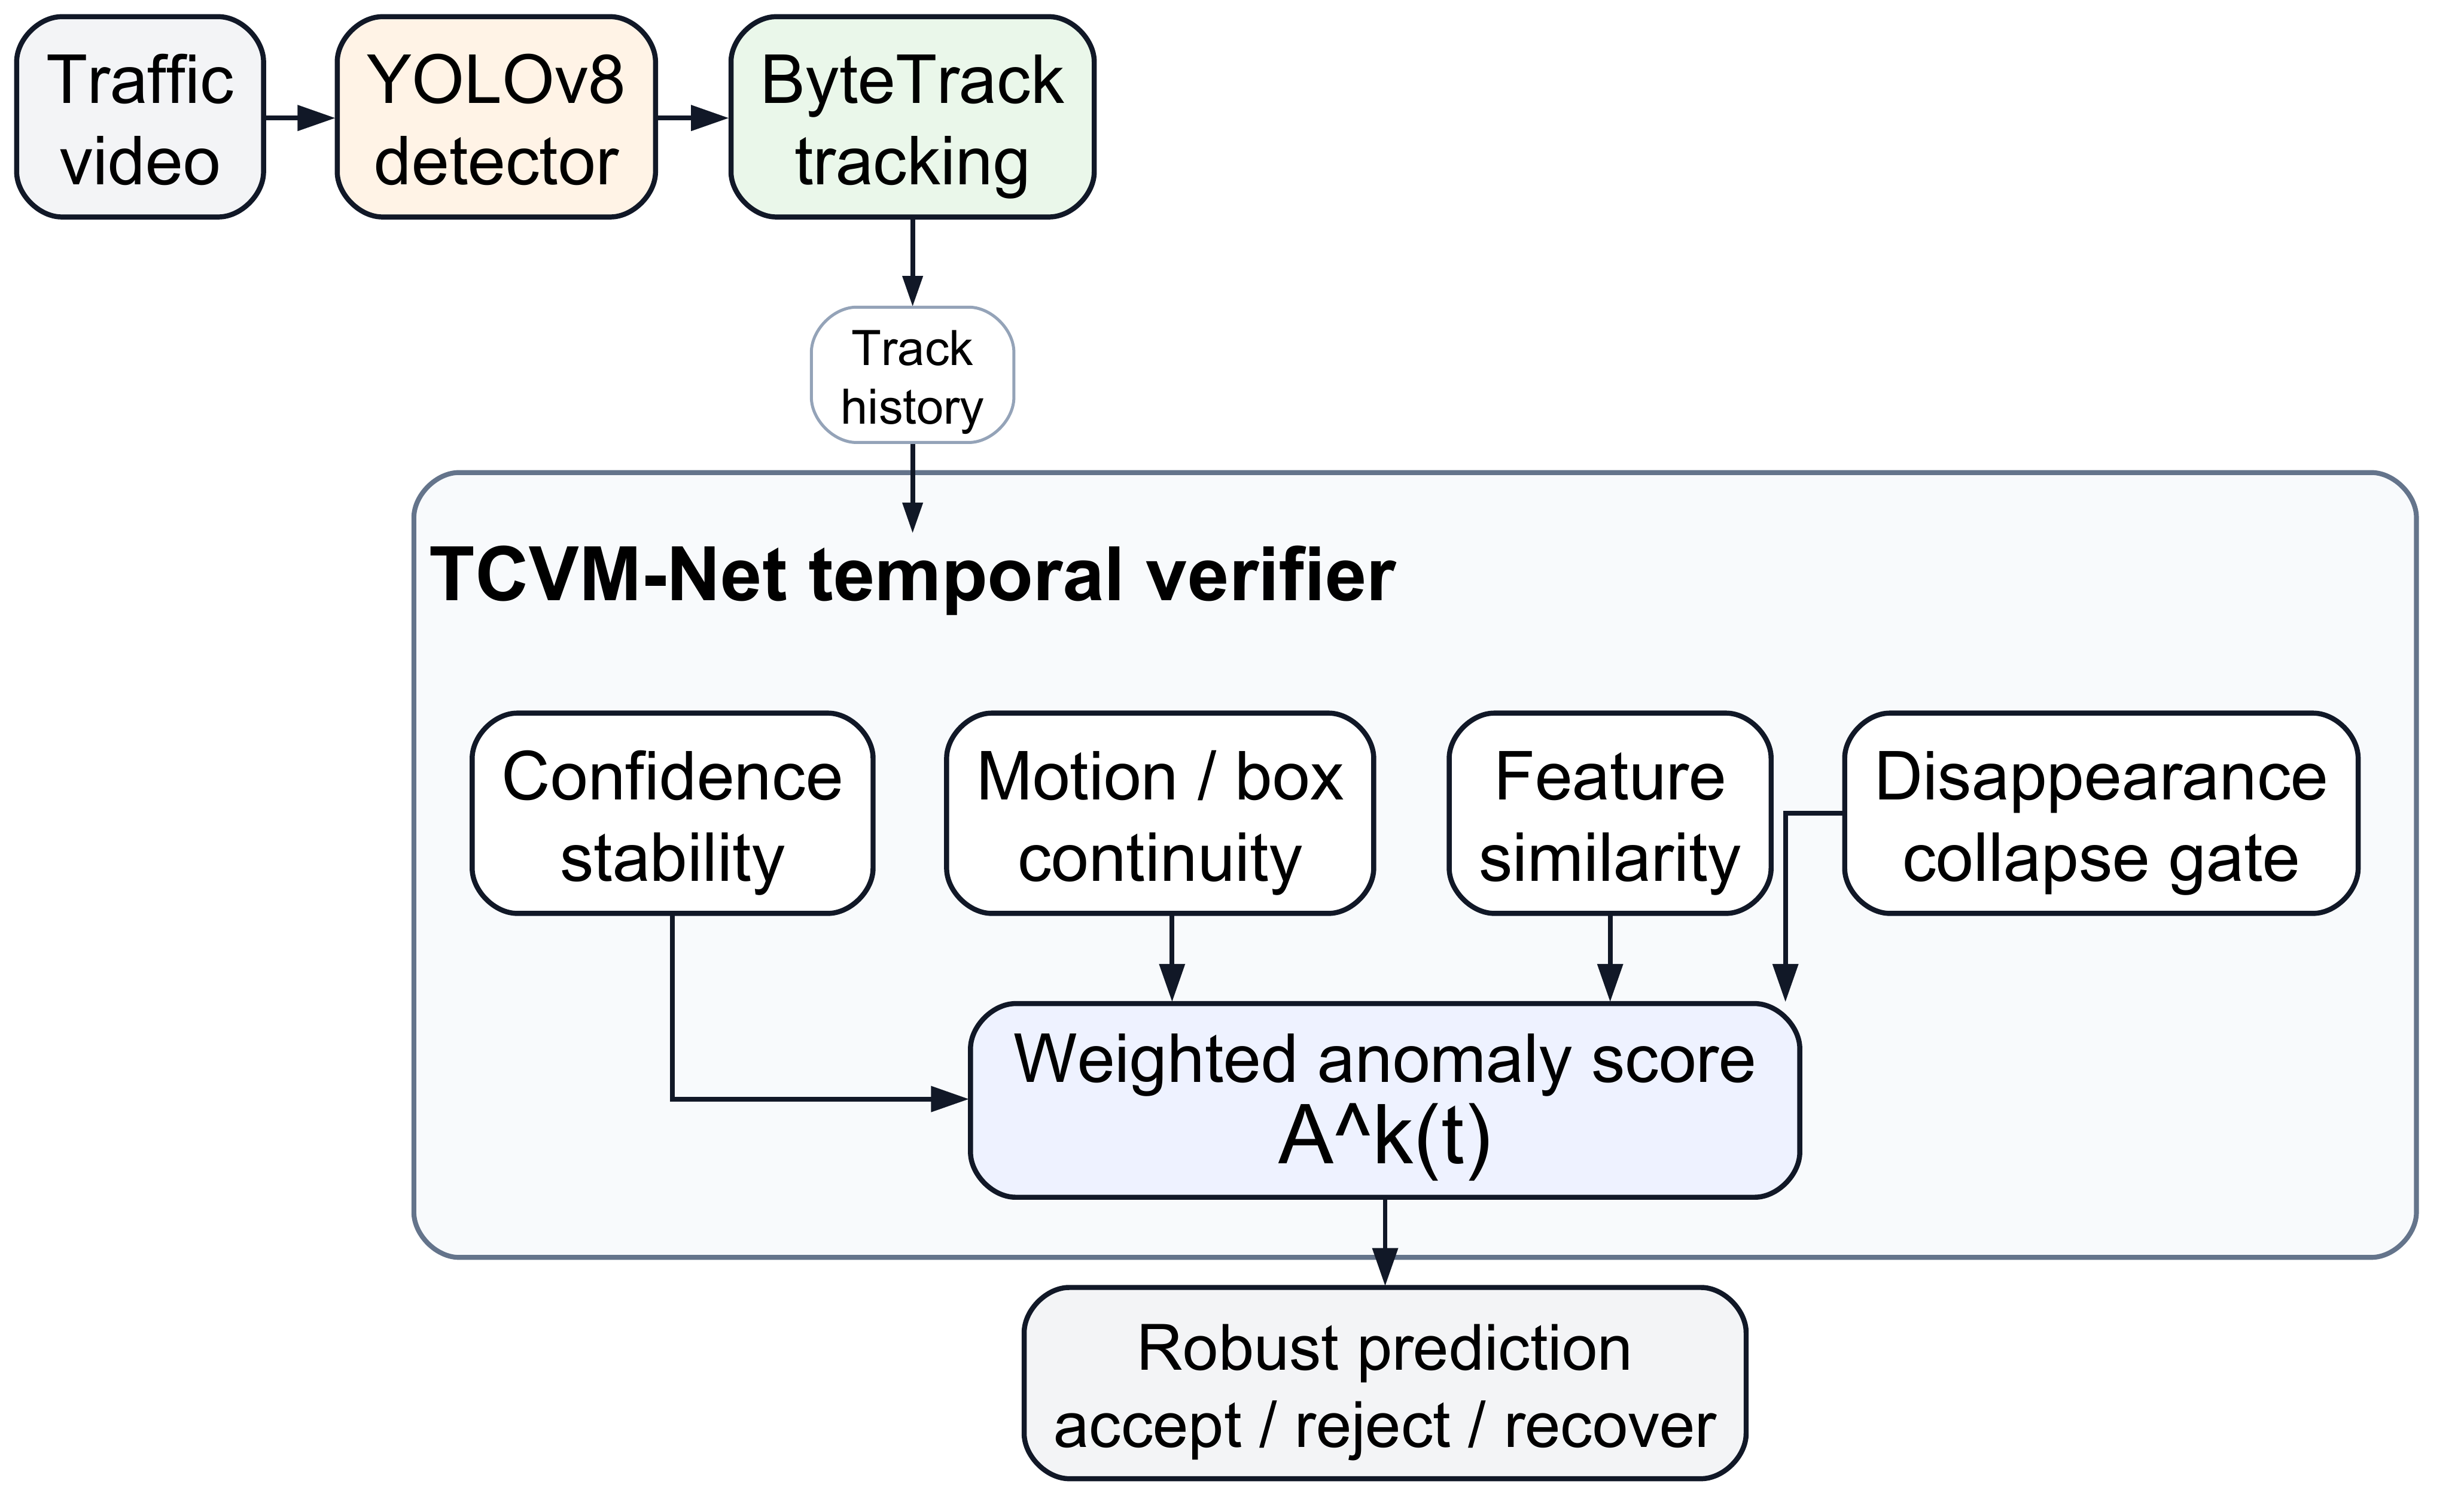
\includegraphics[width=0.96\linewidth]{figures/architecture_graphviz.png}
\caption{YOLOv8+\method{} architecture for temporal adversarial defense in traffic surveillance video.}
\label{fig:architecture}
\end{figure}

Let frame $I_t$ produce detections $\mathcal{D}_t=\{d_t^i\}_{i=1}^{N_t}$. Each detection $d_t^i$ contains bounding box $b_t^i$, class $c_t^i$, confidence $p_t^i$, and appearance embedding $z_t^i$. A tracker maps detections to track identifiers $k$. For each active track, \method{} stores the last $W$ tuples $(b_{\tau}^k,p_{\tau}^k,z_{\tau}^k)$ as a short temporal history.

\subsection{Why Temporal Inconsistency is Security Evidence}
Adjacent frames constrain plausible detector changes without assuming that traffic objects are static. A helmet may translate, scale, or become partially occluded, but a high-confidence track should not vanish for one frame and reappear at nearly the same location without visual cause. Local perturbations can produce confidence collapse, box drift, feature discontinuity, or brief disappearance while the object remains visible. \method{} treats agreement among cues as evidence and recovers only over short reliable histories. The threat model covers localized helmet/rider/vehicle perturbations in ordered video. It does not claim robustness to an adaptive attacker that explicitly optimizes a temporally smooth patch against the verifier.

\subsection{Confidence Stability Analysis}
Abrupt detector-confidence changes can reveal an attack even when the tracked object remains visible. For each track $k$, \method{} maintains an exponential moving confidence mean $\mu_{t-1}^k$ and variance $(\sigma_{t-1}^k)^2$:
\begin{equation}
s_c^k(t)=
\min\left(1,\frac{|p_t^k-\mu_{t-1}^k|}
{\tau_c(\sigma_{t-1}^k+\epsilon)}\right),
\end{equation}
where $\tau_c$ controls natural variation and $\epsilon$ ensures stability.

\subsection{Motion Continuity Verification}
With constant-velocity prediction $\hat{b}_t^k=b_{t-1}^k+(b_{t-1}^k-b_{t-2}^k)$, motion inconsistency is
\begin{equation}
s_m^k(t)=\min\left(1,\frac{1-\operatorname{IoU}(b_t^k,\hat{b}_t^k)}{\tau_m}\right).
\end{equation}
This term penalizes localization changes inconsistent with recent track velocity while tolerating smooth translation and scale variation.

\subsection{Inter-Frame Feature Similarity}
\method{} uses HSV color and Sobel orientation histograms instead of another pretrained embedding network. This choice preserves appearance sensitivity while limiting memory and inference overhead. For descriptor $z_t^k$ and track average $\bar{z}_{t-1}^k$, feature discontinuity is
\begin{equation}
s_f^k(t)=
\min\left(1,\frac{1-\cos(z_t^k,\bar{z}_{t-1}^k)}{2\tau_f}\right).
\end{equation}
This captures abrupt local appearance change caused by stickers or reflective patterns at low cost.

\subsection{Disappearance Consistency}
For an unmatched, recently confident track $k$, the missing-track score is
\begin{equation}
s_d^k(t)=
\min\left(1,\frac{m_t^k}{M}\right)\mathbf{1}[\mu_{t-1}^k>\gamma],
\end{equation}
where $m_t^k$ counts consecutive misses, $M$ is the patience window, and $\gamma$ is the recovery confidence floor.

An isolated unmatched track may reflect an ordinary ID switch or occlusion rather than an attack. To suppress such recovery, let $U_t$ denote unmatched recent tracks and gate recovery on detector-count collapse:
\begin{equation}
g_t=\mathbf{1}\left[U_t\geq U_{\min}\right]
\mathbf{1}\left[\frac{N_t}{N_t+U_t+\epsilon}\leq\rho\right].
\end{equation}
Only missing events with $g_t=1$ and sufficient disappearance score are recovered, tying intervention to a frame-level failure pattern rather than single-track noise.

\subsection{Temporal Anomaly Score and Recovery}
The final temporal anomaly score is
\begin{equation}
A^k(t)=w_c s_c^k(t)+w_m s_m^k(t)+w_f s_f^k(t)+w_d s_d^k(t),
\quad \sum_i w_i=1.
\end{equation}
When $A^k(t)\geq\theta$, the prediction is flagged and recovered from the temporal prior:
\begin{equation}
\tilde{y}_t^k=
\begin{cases}
y_t^k, & A^k(t)<\theta,\\
(\hat{b}_t^k,c_{t-1}^k,\lambda\mu_{t-1}^k), & A^k(t)\geq\theta,
\end{cases}
\end{equation}
Here $\lambda<1$ discounts recovered confidence. Recovered predictions do not aggressively update history, limiting feedback poisoning. The causal sequence is detection, association, scoring, accept/reject/recover, and conservative history update; no future frame is used.

For $K_t$ active tracks and fixed history length $W$, scalar confidence, motion, and anomaly updates are linear in $K_t$; history storage is $O(K_tW)$. Descriptor extraction is restricted to detected regions, and optical flow is optional and resolution-scalable. The verifier performs no gradient update or secondary-network inference, so its principal adjustable cost is image-space flow rather than learned-model memory.

\section{Datasets and Benchmark Protocol}

Public data were obtained with the Kaggle CLI; URLs, checksums, seeds, split files, and configurations are recorded. Hard Hat Detection XML annotations were converted to YOLO helmet, no-helmet, and rider classes and checked for invalid or out-of-frame boxes. The 3500/750/750 train/validation/test split contains 25502 valid boxes; the held-out test set has 2781 helmet, 899 no-helmet, and 78 rider instances.

Validated BDD100K \cite{yu2020bdd100k} adds 70000/10000/20000 train/validation/test traffic images across person, rider, vehicle, and traffic-control classes; class statistics use 5000 sampled labels per split.

\dataset{} merges these sources into an attack-ready YOLO structure. Detector experiments use the helmet split; temporal tests deliberately span three evidence levels: a controlled reflective probe with clean labels, a natural-motion Kaggle video with clean YOLOv8 pseudo-labels, and 30 video-disjoint public HELMET clips with 720 human-annotated frames and 5577 motorcycle boxes. Five attacks affect identical three-frame windows; ten clips calibrate the threshold on occlusion only and twenty remain held out for cross-attack reporting.

All perturbations are generated after data splitting, and each attacked image retains its clean annotation for paired evaluation. Video clips, rather than adjacent frames, define calibration/test membership to prevent temporal leakage. Threshold selection uses only anomaly labels from the calibration clips; detector metrics and held-out anomaly scores are then computed with the selected value frozen.

\subsection{Attack Generation}
We evaluate FGSM, PGD, patch, sticker, reflective, occlusion, motion-blur, and low-light attacks. Native-gradient FGSM and PGD minimize the mean score of the top 1\% target-class anchors under an $\ell_\infty$ budget. The attack variable remains on the native image grid, is differentiably resized to $640\times640$, and uses target-class probabilities from YOLOv8's decoded $[B,4+C,N]$ output. Localized attacks randomize scale, position, and illumination near helmet or rider boxes. A printability-constrained EOT patch is optimized directly against YOLOv8 motorcycle confidence using one image from each calibration clip, then frozen for held-out evaluation. These digital overlays test detector-specific persistence but are not presented as printed evidence.

Executed budgets are FGSM $\epsilon=8/255$ and 10-step PGD with $\epsilon=8/255$, step size $2/255$, and random initialization. The generic patch is $96\!\times\!96$ pixels at 0.45 target-box scale; sticker scale is 0.38. Reflective stripes use intensity 0.82 and width 8; occlusion covers 0.35 of each target; motion blur uses a 17-pixel kernel; and low light uses $\gamma=1.8$ with gain 0.72. The detector-specific patch uses the same size and scale, 30 optimization steps, learning rate 0.05, ten clip-disjoint optimization images, and 720 evaluation frames.

\section{Experimental Setup}

\subsection{Baselines}
The experiments compare:
\begin{enumerate}
    \item YOLOv8n and YOLOv8s baselines trained on clean helmet frames.
    \item An adversarial-augmentation YOLOv8n baseline trained with clean frames plus generated attack samples.
    \item Image-only preprocessing with JPEG recompression, median filtering, and CLAHE.
    \item ADAV-style reference-frame recovery and YOLOv8+\method{} temporal verification.
\end{enumerate}
Adversarial augmentation fine-tunes the clean YOLOv8n checkpoint on clean data plus 300 images per attack family. The ADAV-style comparator is not a reproduction: it flags disappearance against stable reference boxes and recovers them with decayed confidence.

\subsection{Metrics}
Metrics are mAP@50, mAP@50:95, attack success rate (ASR), robust accuracy, anomaly accuracy/precision/recall/F1/FPR, FPS, mean and p95 latency, memory, and GPU utilization. ASR is the fraction of clean-detected targets suppressed by attack, and robust accuracy is its complement for that target set. Anomaly metrics are frame-level; detection metrics remain box-level. Runtime uses batch size one and includes detector plus enabled verifier operations.

\subsection{Implementation Details}
YOLOv8n was trained for 50 epochs at 640 pixels, batch 32, mixed-precision CUDA, early stopping, and fixed seeds; YOLOv8s used the same protocol. AdvAug-YOLOv8n stopped at epoch 44 (best 29). Attack generation uses seed 2026, and robustness rows use the same 50 filenames for clean and perturbed evaluation. All attacks and temporal tests defend YOLOv8n. The probe uses $W=8$, $\alpha=0.35$, $(w_c,w_m,w_f,w_d)=(0.34,0.28,0.26,0.12)$, $(U_{\min},\rho)=(2,0.35)$, and $\theta=0.45$. Public HELMET selects $\theta$ on ten occlusion calibration clips by maximizing F1 subject to recall $\geq0.70$ and FPR $\leq0.10$, then freezes it for twenty clips and every other attack. Table~\ref{tab:baseline_models_auto} reports clean held-out detection performance for the trained baselines.

\IfFileExists{tables/baseline_models_auto.tex}{\begin{table}[t]
\caption{Clean held-out test performance of trained YOLOv8 helmet baselines.}
\label{tab:baseline_models_auto}
\small
\setlength{\tabcolsep}{3.5pt}
\resizebox{\linewidth}{!}{%
\begin{tabular}{lrrrrrr}
\toprule
Model & Epochs & mAP@50 & mAP@50:95 & Precision & Recall & Inference (ms) \\
\midrule
YOLOv8n & 50 & 0.628 & 0.415 & 0.610 & 0.617 & 3.025 \\
YOLOv8s & 50 & 0.634 & 0.417 & 0.957 & 0.593 & 5.908 \\
AdvAug-YOLOv8n & 44 & 0.623 & 0.404 & 0.610 & 0.586 & 3.473 \\
\bottomrule
\end{tabular}%
}
\end{table}
}{\PackageError{tcvm}{Missing generated baseline table}{Regenerate the baseline table from validated experiment outputs.}}

\section{Results and Discussion}

Table~\ref{tab:robustness_auto} evaluates a paired subset of 50 held-out helmet images against the final checkpoint. Clean mAP@50 is 0.675 on those same images. FGSM and PGD reach ASR 0.473 [0.382, 0.558] and 0.988 [0.972, 1.000], lowering mAP@50 to 0.337 and 0.229. Reflective, occlusion, and blur reach ASR 0.863 [0.788, 0.945], 0.801 [0.724, 0.884], and 0.672 [0.543, 0.781]. Image preprocessing recovers FGSM and PGD mAP@50 to 0.513 and 0.662 and helps occlusion and sticker, but lowers reflective mAP@50 from 0.152 to 0.100.

\IfFileExists{tables/robustness_auto.tex}{\begin{table}[t]
\caption{Robustness on the paired 50-image subset. Base ASR and robust target accuracy (RAcc.) quantify the unmitigated attack and are repeated across methods; mitigation is compared by mAP.}
\label{tab:robustness_auto}
\small
\setlength{\tabcolsep}{3.5pt}
\resizebox{\linewidth}{!}{%
\begin{tabular}{llrrrr}
\toprule
Attack & Method & Base ASR & Base RAcc. & mAP@50 & mAP@50:95 \\
\midrule
Clean & YOLOv8 & 0.000 & 1.000 & 0.675 & 0.471 \\
FGSM & YOLOv8 & 0.473 & 0.527 & 0.337 & 0.166 \\
FGSM & Image-only & 0.473 & 0.527 & 0.513 & 0.318 \\
PGD & YOLOv8 & 0.988 & 0.012 & 0.229 & 0.118 \\
PGD & Image-only & 0.988 & 0.012 & 0.662 & 0.448 \\
Patch & YOLOv8 & 0.390 & 0.610 & 0.407 & 0.219 \\
Patch & Image-only & 0.390 & 0.610 & 0.440 & 0.245 \\
Sticker & YOLOv8 & 0.261 & 0.739 & 0.505 & 0.295 \\
Sticker & Image-only & 0.261 & 0.739 & 0.566 & 0.341 \\
Reflective & YOLOv8 & 0.863 & 0.137 & 0.152 & 0.076 \\
Reflective & Image-only & 0.863 & 0.137 & 0.100 & 0.049 \\
Motion blur & YOLOv8 & 0.672 & 0.328 & 0.246 & 0.106 \\
Motion blur & Image-only & 0.672 & 0.328 & 0.283 & 0.125 \\
Occlusion & YOLOv8 & 0.801 & 0.199 & 0.216 & 0.125 \\
Occlusion & Image-only & 0.801 & 0.199 & 0.321 & 0.194 \\
Low light & YOLOv8 & 0.029 & 0.971 & 0.651 & 0.445 \\
Low light & Image-only & 0.029 & 0.971 & 0.646 & 0.441 \\
\bottomrule
\end{tabular}%
}
\end{table}
}{\PackageError{tcvm}{Missing generated robustness table}{Regenerate the robustness table from validated experiment outputs.}}

Attack specificity is central. PGD gives the highest target-suppression ASR, whereas reflective perturbation gives the lowest detector mAP@50 because ASR counts disappearance of clean-matched targets while mAP also measures class-wide precision and localization. Image preprocessing is effective for the tested norm-bounded perturbations but inconsistent for physical-style corruptions; low light is largely benign at the executed intensity, while reflective and occlusion attacks remain severe. Temporal analysis therefore emphasizes reflective failures, where framewise preprocessing is weakest and disappearance is interpretable across adjacent frames.

Matched adversarial augmentation (Table~\ref{tab:adversarial_training_auto}) raises FGSM and PGD mAP@50 from 0.337 to 0.420 and from 0.229 to 0.540; reflective and occlusion increase from 0.152 to 0.910 and from 0.216 to 0.918. On the full 750-image test set, its clean mAP@50 is 0.623 versus 0.628 for YOLOv8n (Table~\ref{tab:baseline_models_auto}); the paired 50-image subset instead shows 0.699 versus 0.675, illustrating subset variation. The large matched-family gains show that these generated corruptions are learnable when represented during training. They should not be interpreted as open-world physical robustness; \method{} instead targets the orthogonal failure mode of abrupt video-level inconsistency after inference.

\IfFileExists{tables/adversarial_training_auto.tex}{\begin{table}[t]
\caption{Adversarial augmentation on the paired 50-image attack splits; entries are mAP.}
\label{tab:adversarial_training_auto}
\small
\setlength{\tabcolsep}{3.5pt}
\resizebox{\linewidth}{!}{%
\begin{tabular}{lrrrrr}
\toprule
Attack & Base @50 & AdvAug @50 & $\Delta$ @50 & Base @50:95 & AdvAug @50:95 \\
\midrule
Clean & 0.675 & 0.699 & 0.023 & 0.471 & 0.464 \\
FGSM & 0.337 & 0.420 & 0.084 & 0.166 & 0.223 \\
PGD & 0.229 & 0.540 & 0.311 & 0.118 & 0.335 \\
Patch & 0.407 & 0.963 & 0.557 & 0.219 & 0.741 \\
Sticker & 0.505 & 0.958 & 0.453 & 0.295 & 0.734 \\
Reflective & 0.152 & 0.910 & 0.759 & 0.076 & 0.782 \\
Motion blur & 0.246 & 0.572 & 0.326 & 0.106 & 0.348 \\
Occlusion & 0.216 & 0.918 & 0.702 & 0.125 & 0.710 \\
Low light & 0.651 & 0.655 & 0.004 & 0.445 & 0.442 \\
\bottomrule
\end{tabular}%
}
\end{table}
}{\PackageError{tcvm}{Missing generated adversarial-training table}{Regenerate the adversarial-training table from validated experiment outputs.}}

\subsection{Temporal Consistency Analysis}
A controlled 24-frame probe uses a held-out image with 38 helmet targets; frames 8--11 receive reflective perturbations while retaining clean boxes. YOLOv8 obtains 0.838/0.581 mAP@50/50:95; recovery raises these to 0.944/0.664. Frame-level anomaly accuracy, precision, recall, F1, and FPR are 0.958, 1.000, 0.750, 0.857, and 0.000.

The reflective pattern causes frame-local failure while track history remains plausible. Rather than classify the perturbation, \method{} detects a departure from prior confidence and continuity after inference. This distinction explains why recovery is effective for transient collapse but cannot guarantee detection of a persistent patch that changes the track smoothly.

An 80-frame Kaggle helmet sequence, sampled every five frames, tests natural motion and dense traffic. Clean YOLOv8 produces 1037 pseudo-labels before a reflective attack over frames 30--46. This is not human-annotated attacked video; \method{} raises pseudo-label mAP@50 from 0.432 to 0.522 at $\theta=0.45$ (Table~\ref{tab:real_video_auto}), with partial anomaly calibration.

\IfFileExists{tables/real_video_auto.tex}{\begin{table}[t]
\centering
\caption{Real-video reflective stress test using clean YOLOv8 pseudo-labels rather than human annotations.}
\label{tab:real_video_auto}
\small
\setlength{\tabcolsep}{4pt}
\begin{tabular}{lrrrrr}
\toprule
Method & $\theta$ & mAP@50 & mAP@50:95 & Anom. Acc. & FPS \\
\midrule
YOLOv8 baseline & \multicolumn{1}{c}{n/a} & 0.432 & 0.407 & \multicolumn{1}{c}{n/a} & \multicolumn{1}{c}{n/a} \\
YOLOv8+\method{} & 0.45 & 0.522 & 0.512 & 0.713 & 13.73 \\
\bottomrule
\end{tabular}
\end{table}
}{\PackageError{tcvm}{Missing generated real-video table}{Run the real-video TCVM benchmark.}}

Thirty public HELMET clips with human motorcycle boxes receive identical three-frame attack windows. Ten clips select $\theta=0.70$ using occlusion only; the threshold is then frozen for twenty clips and four unseen attack families. Occlusion lowers COCO YOLOv8n mAP@50 from 0.457 to 0.388 and reaches held-out F1/recall/FPR of 0.887/0.917/0.021. Without retuning, reflective attack obtains the same operating point and similar mAP loss (Table~\ref{tab:public_helmet_crossattack_auto}). Across 20 fixed clip-disjoint resplits, $\theta=0.70$ is selected 17 times and $0.60$ three times; held-out F1 has median 0.889 (IQR 0.880--0.907) and median FPR 0.020.

\IfFileExists{tables/public_helmet_crossattack_frozen070_auto.tex}{\begin{table}[t]
\caption{Frozen-threshold cross-attack evaluation on 20 held-out HELMET clips. $\theta=0.70$ is selected only on disjoint occlusion calibration clips; mAP uses all 720 frames and anomaly metrics use the 480 held-out frames.}
\label{tab:public_helmet_crossattack_auto}
\small
\setlength{\tabcolsep}{3.2pt}
\resizebox{\linewidth}{!}{%
\begin{tabular}{lrrrrrr}
\toprule
Attack & YOLO mAP@50 & TCVM mAP@50 & $\Delta$ mAP & Held-out Rec. & Held-out F1 & Held-out FPR \\
\midrule
Occlusion & 0.388 & 0.394 & 0.006 & 0.917 & 0.887 & 0.021 \\
Reflective & 0.388 & 0.393 & 0.006 & 0.917 & 0.887 & 0.021 \\
Detector patch & 0.427 & 0.428 & 0.001 & 0.067 & 0.103 & 0.033 \\
Sticker & 0.453 & 0.449 & -0.005 & 0.000 & 0.000 & 0.036 \\
Motion blur & 0.449 & 0.445 & -0.004 & 0.000 & 0.000 & 0.031 \\
\bottomrule
\end{tabular}%
}
\end{table}
}{\PackageError{tcvm}{Missing public HELMET cross-attack table}{Run the frozen-threshold cross-attack benchmark.}}

The detector patch is optimized on one image from each calibration clip. On the twenty disjoint clips, an all-frame overlay suppresses 0.406 of clean-detected targets; short-gap application lowers mAP@50 to 0.427 but reaches only 0.103 anomaly F1. Sticker and 17-pixel blur alter mAP@50 by less than 0.009 and trigger no attack-window detections. Thus, \method{} is neither a generic corruption classifier nor robust to temporally smooth patches.

With thresholds frozen at 0.70/0.85, \method{} versus ADAV-style reference recovery reaches F1/FPR of 0.887/0.021 versus 0.870/0.012 on occlusion, and 0.887/0.021 versus 0.839/0.012 on reflective attack (Table~\ref{tab:crossattack_temporal_baselines}). Tracker-only recovery reaches only 0.318 F1 at 0.612 FPR. \method{} and reference recovery fail on the optimized patch and weak sticker/blur settings; tracker-only responses are dominated by false positives. These outcomes bound the robustness claim to abrupt temporal failures.

\IfFileExists{tables/crossattack_temporal_baselines_frozen_auto.tex}{\begin{table}[tbp]
\caption{Frozen temporal-baseline transfer on the 20 held-out HELMET clips. Entries are anomaly F1/FPR; no attack-specific threshold tuning is used.}
\label{tab:crossattack_temporal_baselines}
\scriptsize
\centering
\setlength{\tabcolsep}{4pt}
\begin{tabular}{lccc}
\toprule
Attack & TCVM-Net & Track recovery & Reference recovery \\
\midrule
Occlusion & 0.887/0.021 & 0.318/0.612 & 0.870/0.012 \\
Reflective & 0.887/0.021 & 0.318/0.612 & 0.839/0.012 \\
Detector patch & 0.103/0.033 & 0.227/0.693 & 0.088/0.012 \\
Sticker & 0.000/0.036 & 0.223/0.710 & 0.000/0.012 \\
Motion blur & 0.000/0.031 & 0.219/0.690 & 0.000/0.012 \\
\bottomrule
\end{tabular}
\end{table}
}{\PackageError{tcvm}{Missing cross-attack temporal-baseline table}{Run the frozen temporal-baseline benchmark.}}

\begin{figure}[tbp]
\centering
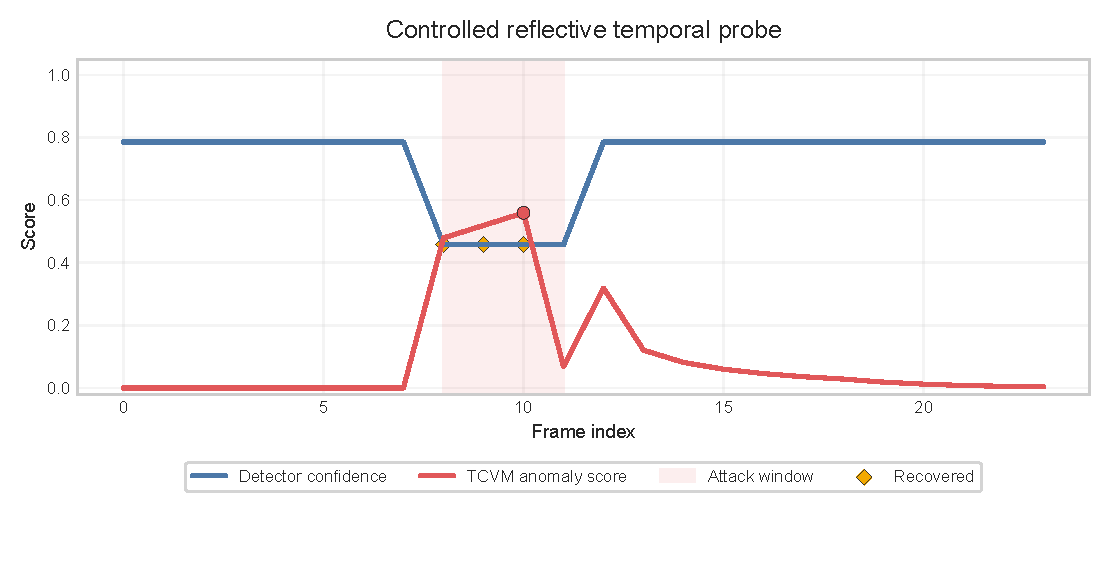
\includegraphics[width=\linewidth]{../outputs/figures/temporal_confidence_reflective_probe.pdf}
\caption{Temporal confidence and anomaly trajectory on the reflective probe. Detector confidence collapses during the attack window, while \method{} produces anomaly spikes and recovers missing tracks.}
\label{fig:temporal_confidence}
\end{figure}

\subsection{Explainability}
Offline Grad-CAM \cite{selvaraju2017grad} shifts under the reflective pattern as detections collapse from 41 to 1 (Fig.~\ref{fig:gradcam}), linking a localized attention change to the confidence and disappearance events observed by \method{}. This is mechanism-oriented evidence rather than proof of causality, and the heatmaps are not used at inference.

\begin{figure}[tbp]
\centering
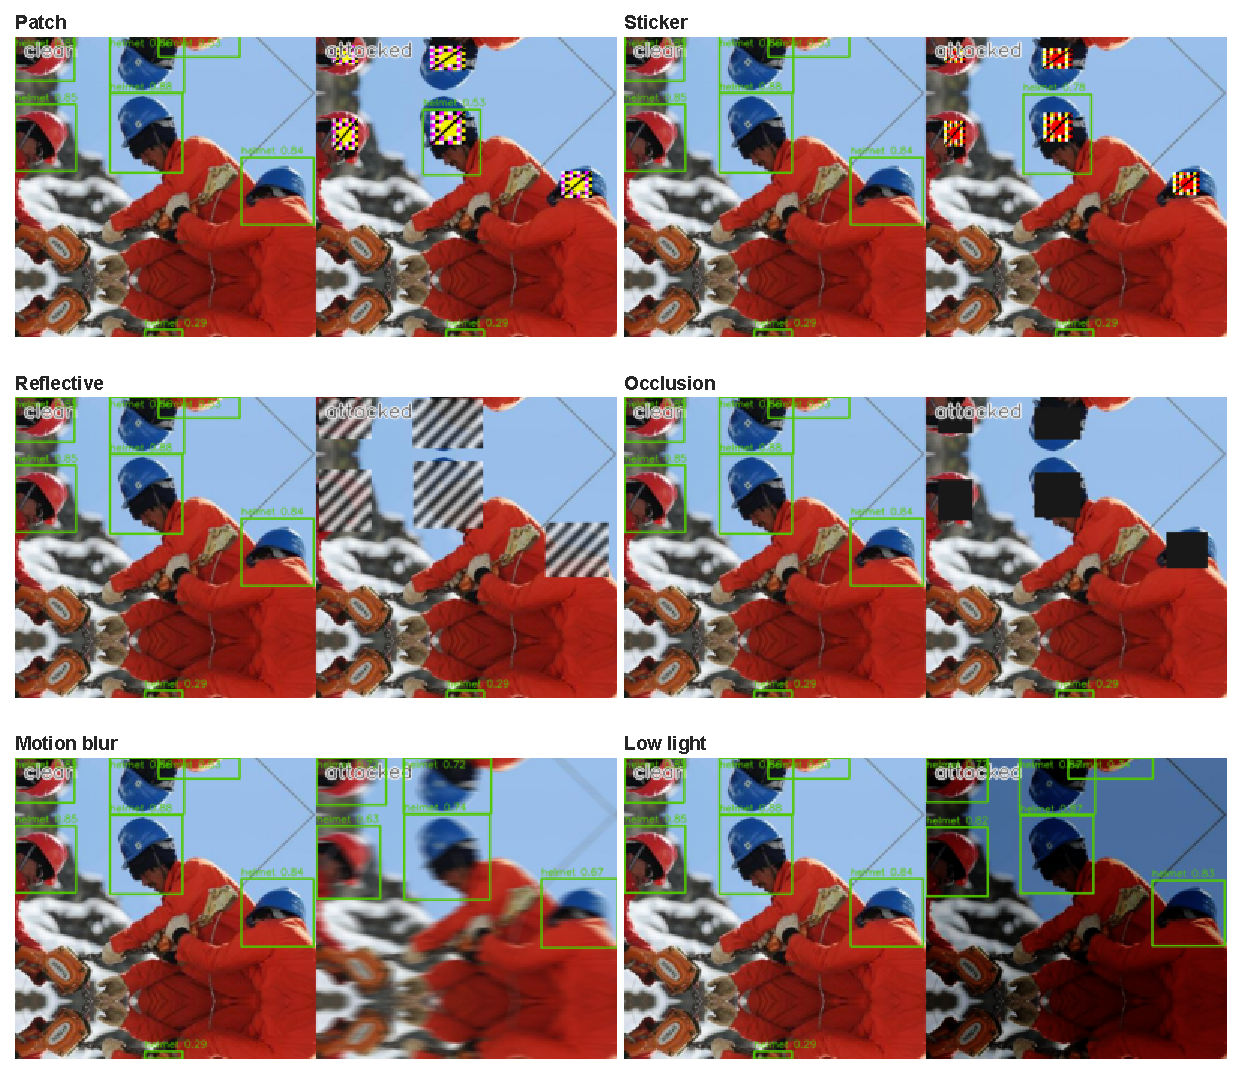
\includegraphics[width=0.86\linewidth]{../outputs/figures/attack_gallery.pdf}
\caption{Representative physical-style attack panels generated by the benchmark pipeline.}
\label{fig:attack_gallery}
\end{figure}

\begin{figure}[tbp]
\centering
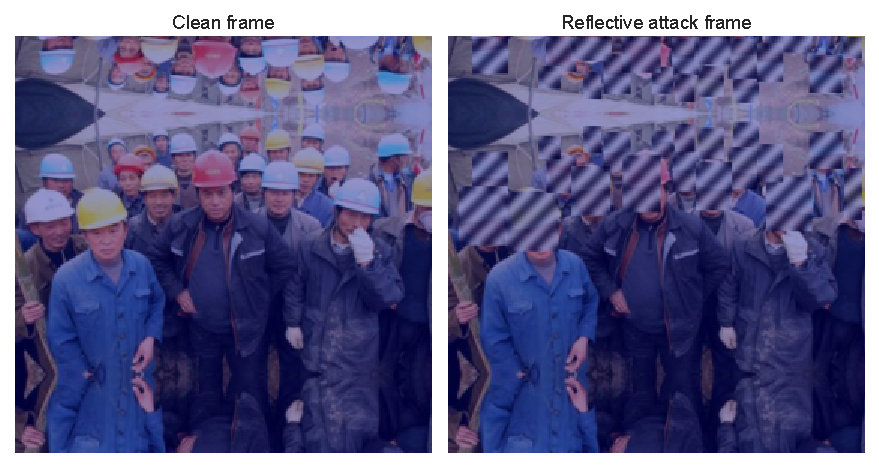
\includegraphics[width=0.86\linewidth]{../outputs/figures/gradcam_reflective_probe/gradcam_comparison.pdf}
\caption{Grad-CAM overlays before and during the reflective temporal attack. The perturbation shifts detector attention while \method{} observes the resulting confidence and disappearance inconsistency.}
\label{fig:gradcam}
\end{figure}

\section{Ablation Studies}

Table~\ref{tab:ablation_auto} evaluates \method{} variants on the original public HELMET 20-clip occlusion benchmark.

\IfFileExists{tables/ablation_auto.tex}{\begin{table}[ht]
\caption{Component ablation on the 20-clip public HELMET occlusion benchmark.}
\label{tab:ablation_auto}
\small
\setlength{\tabcolsep}{3.5pt}
\resizebox{\linewidth}{!}{%
\begin{tabular}{lrrrrr}
\toprule
Variant & mAP@50 & mAP@50:95 & Anom. F1 & FPR & FPS \\
\midrule
Full TCVM & 0.355 & 0.076 & 0.591 & 0.181 & 11.842 \\
Track recovery & 0.365 & 0.078 & 0.307 & 0.645 & 11.410 \\
No confidence & 0.355 & 0.077 & 0.616 & 0.162 & 11.129 \\
No motion & 0.344 & 0.074 & 0.435 & 0.345 & 11.515 \\
No feature & 0.331 & 0.071 & 0.355 & 0.486 & 12.728 \\
No smoothing & 0.354 & 0.075 & 0.567 & 0.200 & 11.969 \\
No recovery & 0.346 & 0.074 & 0.591 & 0.181 & 11.137 \\
\bottomrule
\end{tabular}%
}
\end{table}
}{\PackageError{tcvm}{Missing generated ablation table}{Regenerate the ablation table from validated experiment outputs.}}

On the original 20-clip ablation, \method{} reaches 0.591 F1 and 0.181 FPR versus 0.307/0.645 for tracker-only recovery. Reference recovery reaches 0.938/0.000 on that full-box occlusion setting, confirming previous-frame consistency as a strong but narrower comparator; the disjoint 30-clip comparison in Table~\ref{tab:crossattack_temporal_baselines} is less favorable and tests attack transfer. Removing motion, feature, or smoothing lowers F1 to 0.435, 0.355, or 0.567. Removing recovery preserves anomaly F1 but lowers mAP@50 from 0.355 to 0.346. Removing confidence slightly improves F1 on this occlusion-only benchmark, showing that confidence stability is attack-family dependent rather than uniformly beneficial.

On the reflective probe, disabling recovery drops mAP@50 from 0.944 to 0.828. Together, the controlled and public-video tests support the bounded claim that recovery restores short collapses while motion, feature, and smoothing suppress tracker-only false alarms. They do not establish superiority to reference recovery for every disappearance attack.

\section{Edge Deployment Analysis}

\IfFileExists{tables/edge_auto.tex}{\begin{table}[H]
\caption{Edge deployment latency, throughput, and memory usage.}
\label{tab:edge_auto}
\small
\setlength{\tabcolsep}{3.5pt}
\resizebox{\linewidth}{!}{%
\begin{tabular}{lrrrr}
\toprule
Method & Mean Latency (ms) & p95 Latency (ms) & FPS & Peak RSS (MB) \\
\midrule
YOLOv8 & 117.776 & 154.312 & 8.491 & 1102.188 \\
YOLOv8+TCVM-Net & 251.183 & 294.108 & 3.981 & 1120.465 \\
\bottomrule
\end{tabular}%
}
\end{table}
}{\PackageError{tcvm}{Missing generated edge table}{Regenerate the edge table from validated experiment outputs.}}

On an RTX 4060 Laptop GPU, the controlled probe runs at 8.49 FPS for YOLOv8 and 3.98 FPS with \method{}, while resident memory rises from 1102 to 1120 MB (Table~\ref{tab:edge_auto}). Profiling identifies dense optical flow, rather than model memory, as the principal cost. Quarter-flow reaches 14.10 FPS and 0.891 F1 on the calibrated 30-clip benchmark; full-resolution flow exhausted OpenCV memory in an earlier 480-frame run. Full verification therefore suits selective streams, while scaled/no-flow modes trade detection quality for throughput. These measurements establish laptop feasibility, not Jetson performance.

\section{Discussion and Limitations}

\method{} requires ordered frames and reliable short tracks; camera shake, extreme blur, long occlusion, reflective saturation, ID switches, and abrupt viewpoint changes weaken temporal evidence. Thresholds remain camera- and class-dependent: clip-disjoint calibration helps public HELMET, while uncalibrated $\theta=0.30$ over-flags the Kaggle video. Validation is bounded by one clean-label probe, pseudo-labels, synthetic attack windows on annotated public video, and modest mAP recovery in the hardest setting. Persistent optimized patches can also remain temporally smooth, exposing a synthetic-to-real and adaptive-attack gap. Printed perturbations, broader multi-camera data, and structured video attacks remain necessary before deployment. Operational use should retain local calibration, audit logs, and human review rather than automatic enforcement.

\section{Conclusion and Future Work}

\method{} converts confidence, motion, appearance, count collapse, and disappearance continuity into a lightweight YOLOv8 verification signal. Experiments demonstrate physical-style vulnerabilities, split-stable calibration, short-collapse recovery, frozen-threshold transfer to reflective attacks, and failure on temporally smooth detector patches. Future work targets adaptive attacks, multi-camera consistency, video detectors, and printed hardware-in-the-loop tests.

\begingroup
\bibliographystyle{splncs04}
\bibliography{references}
\endgroup

\end{document}
